The basic abstraction of the \gls{lsm} interface is to intercede in the access to internal kernel objects. Security modules should answer a simple question "May a subject \texttt{S} perform a kernel operation \texttt{OP} on an internal kernel object \texttt{OBJ}?". The mechanism that allow modules to execute this task lies in \textit{hook} functions that are placed in the kernel code, as shown in \autoref{fig:lsm_arch}.

\begin{figure}[htbp]
 \centering
 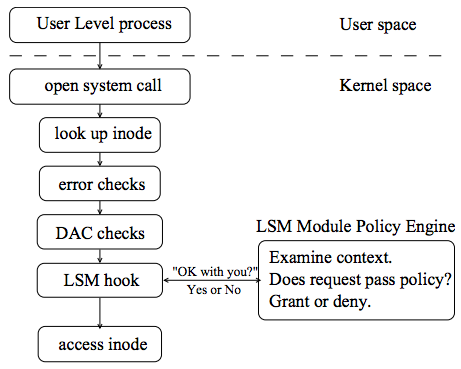
\includegraphics[scale=0.5]{images/LSM_architecture.png}
 \caption{LSM hook functions architecture}
 \label{fig:lsm_arch}
\end{figure}

\noindent
Immediately before the kernel access the object, represented as \textit{inode} in \autoref{fig:lsm_arch}, the hook makes a call to a function that the \gls{lsm} must provide. The module, based on policy rules, either allow or deny the access, forcing an error code return in the last case.
